\documentclass{standalone}
\usepackage[T1]{fontenc}
\usepackage[utf8]{inputenc}
\usepackage{pgf,tikz}
\usepackage{setspace}
\usepackage{pgfplots}
\pgfplotsset{compat=1.12}

\begin{document}


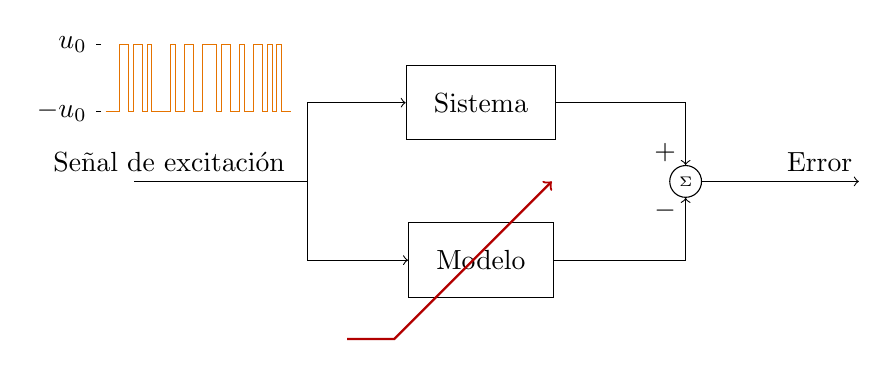
\begin{tikzpicture}[node distance=22mm, block/.style={rectangle, draw, minimum width=15mm, inner sep=10pt}, sumnode/.style={circle, draw, inner sep=2pt},]
    
       \node[coordinate] (input) {};
       \node[coordinate, right of=input] (copy) {};
       \node[coordinate, right of=copy] (midp) {};
       \node[block, above of=midp, node distance=10mm] (sys)  {Sistema};
       \node[block, below of=midp, node distance=10mm] (mod)  {Modelo};
       \node[sumnode, right of=midp, node distance=26mm] (sum) {\tiny $\Sigma$};
       \node[coordinate, right of=sum, node distance=22mm] (output) {};

       \draw[-] (input) -- node[above, pos=0.2] {Señal de excitación} (copy);
       \draw[->] (copy) |- node[above] {} (sys);
       \draw[->] (copy) |- node[above] {} (mod);
       \draw[->] (sys) -| node[left, pos=0.9] {$+$} (sum);
       \draw[->] (mod) -| node[left, pos=0.9] {$-$} (sum);
       \draw[->] (sum) -- node[above, near end] {Error} (output);

       \draw[thick, red!70!black, ->] (2.7,-2) -- (3.3,-2) -- (5.3, 0);
       
       \begin{axis}[
       width=4.4cm,
       height=2.6cm,
       xshift=-0.6cm, 
       yshift=0.8cm,
       axis line style = {draw=none},
       tick style={draw=none},
       ytick=\empty,
       xtick=\empty,
       clip=false,
       ]
       \addplot+[ orange!90!black, const plot, no marks, domain=1:41, samples=41] {sign(rand)};

       \draw (axis cs: 0, 1) -- (axis cs: -1, 1) node[left] {$u_0$}; 
       \draw (axis cs: 0, -1) -- (axis cs: -1, -1) node[left] {$-u_0$}; 
     \end{axis}

     \end{tikzpicture}
   \end{document}
   